\section{The Cauchy-Goursat Theorem}
\label{Ch5:Sec:Cauchy-Goursat}

\begin{comment}
Maybe begin with an anecdote - no sooner had we entered Hales's office in Pittsburgh than he asked about how we plan to deform integration contours.

Have 3 subsections.
1. Informal maths
2. Discussion of existing formalisation of closed rectangular case, with emphasis on why we don't have it for other cases (cite Hales's formalisation of the Jordan Curve Theorem in HOL-Light, maybe try and explain why we don't have something similar in Lean)
3. Discussion of our approach to the indefinite case (informally and formally)
Also maybe find better words than closed/open? Because these words are NOT used here in a topological sense, but rather in a very visual sense ("are the two endpoints of the curve the same point or are they not? Does the curve even have two endpoints or does it just have one and then go off to i\infty in the other?")
\end{comment}

There are some areas of mathematics that are notoriously difficult to formalise. Algebra, for example, tends to be easier to formalise than analysis. Within analysis, it tends to be particularly difficult to formalise geometric ideas, and few are as deceptively challenging as the innocent-sounding \JCT. It was not until 2007 that this theorem, proposed in the late 19th Century, was formalised by Tom Hales \cite{JordanCurve} in HOL Light, and to this day, no formalisation exists in Lean. The author had the privilege of meeting Hales in Pittsburgh, USA, in March 2025 to discuss the formalisation of $8$-dimensional sphere packing in Lean, and the very first question Hales asked was what the strategy was to overcome the challenges of not having a Lean formalisation of the Jordan Curve Theorem.

The \JCT\ states that a simple closed curve $C \subset \R^2$, given as the image of a continuous injection from $\mathbb{S}^1$, divides $\R^2 \setminus C$ into a bounded region, known as the \textit{interior} of $C$, and an unbounded region, known as the \textit{exterior} of $C$. This gives us a clear way of stating the all-important holomorphicity condition of the \CGT: a path of integration can usually only be deformed if the integrand is holomorphic in the region enclosed by the two paths, and the \JCT\ defines this region. Viazovska uses versions of the \CGT\ to prove the eigenfunction property and the double zero property (see \Cref{Ch4:Sec:Eig,Ch4:Sec:Double_Zeroes}. Fortunately, in both instances, we have explicit contours. Hence, the regions where we require holomorphicity can both be defined, and it is easy to show the integrands are holomorphic in those regions.

This is a significant simplification because it means we have all the ingredients to \textit{state} the results we require. However, there are still challenges involved in proving them. We give a brief overview of the two cases of interest in the forthcoming subsections.

\subsection{Rectangles}

The following version of the \CGT\ had been \href{https://github.com/leanprover-community/mathlib4/blob/c38c7fde32656c7fa1b2471ed1ae0d50a600f089/Mathlib/Analysis/Complex/CauchyIntegral.lean#L241-L255}{formalised} prior to this project.

\begin{boxtheorem}[Cauchy-Goursat for Rectangles]\label{Ch5:Thm:CauchyGoursat_Bounded_on_off_Countable}
    Suppose $f : \C \to \C$ is a function such that $f(z) \to 0$ as $\Im(z) \to \infty$. Then, for all $x_1, y_1, x_2, y_2 \in \R$, if $f$ is holomorphic at all but countably many $z \in \C$ with $x_1 < \Re(z) < x_2$ and $y_1 < \Im(z) < y_2$ and continuous on the corresponding closed rectangle, then
    \begin{align*}
        \int_{x_1}^{x_2} f\of{x + y_1 i} \diff{x}
        - \int_{x_1}^{x_2} f\of{x + y_2 i} \diff{x}
        + i\int_{y_1}^{y_2} f\of{x_2 + yi} \diff{y}
        - i\int_{y_1}^{y_2} f\of{x_1 + yi} \diff{y} = 0
    \end{align*}
\end{boxtheorem}

The author was able to adapt this to the following unbounded version.

\begin{boxtheorem}[Cauchy-Goursat for Unbounded Contours]\label{Ch5:Thm:CauchyGoursat_Unbounded_on_off_Countable}
    Suppose $f : \C \to \C$ is a function such that $f(z) \to 0$ as $\Im(z) \to \infty$. Then, for all $x_1, x_2, y \in \R$, if $f$ is holomorphic at all but countably many $z \in \C$ with $x_1 < \Re(z) < x_2$ and $y < \Im(z)$ and then
    \begin{align*}
        \int_{y}^{\infty} f\of{x_1 + ti} \, \diff{t}
        = \int_{x_1}^{x_2} f\of{t + yi} \, \diff{t}
        + \int_{y}^{\infty} f\of{x_2 + ti} \, \diff{t}
    \end{align*}
    provided that the integrals along the vertical contours exist.
\end{boxtheorem}

\begin{wrapfigure}[12]{r}{0.4\linewidth}
    \vspace{-0.7em}
    \centering
    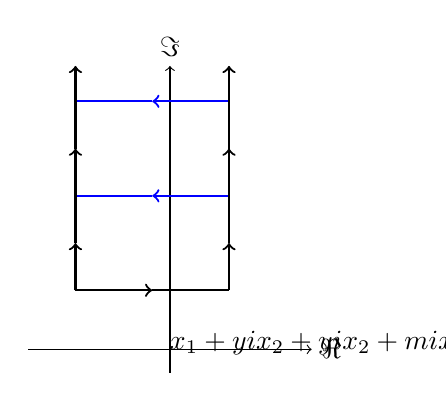
\begin{tikzpicture}[scale=1.5]
        % Axes
        \draw[->] (-1.2,0) -- (1.2,0) node[right] {$\Re$};
        \draw[->] (0,-0.2) -- (0,2.4) node[above] {$\Im$};
    
        % Contours
        % \draw[thick, ->] (-0.8,0.5) -- (-0.8, 2.4);
        % \draw[thick, ->] (0.5,0.5) -- (0.5, 2.4);
        %% Translation Contour
        \draw[thick, ->] (-0.8, 0.5) -- (-0.15, 0.5);
        \draw[thick] (-0.15, 0.5) -- (0.5, 0.5);
        %% Blue vanishing ones
        \draw[thick, blue] (-0.15, 1.3) -- (-0.8, 1.3);
        \draw[thick, ->, blue] (0.5, 1.3) -- (-0.15, 1.3);
        \draw[thick, blue] (-0.15, 2.1) -- (-0.8, 2.1);
        \draw[thick, ->, blue] (0.5, 2.1) -- (-0.15, 2.1);
        %% Vertical ones
        \draw[thick, ->] (-0.8, 0.5) -- (-0.8, 0.9);
        \draw[thick, ->] (0.5, 0.5) -- (0.5, 0.9);
        \draw[thick, ->] (-0.8, 0.9) -- (-0.8, 1.7);
        \draw[thick, ->] (0.5, 0.9) -- (0.5, 1.7);
        \draw[thick, ->] (-0.8, 1.7) -- (-0.8, 2.4);
        \draw[thick, ->] (0.5, 1.7) -- (0.5, 2.4);
    
        % Points of interest
        \labelledpoint{-0.8}{0.5}{-0.8}{-0.3}{$x_1 + yi$}
        \labelledpoint{0.5}{0.5}{0.8}{-0.3}{$x_2 + yi$}
        \labelledpoint{0.5}{1.3}{0.8}{-0.3}{$x_2 + mi$}
        \labelledpoint{0.5}{2.1}{0.8}{-0.3}{$x_2 + mi$}
        \labelledpoint{-0.8}{1.3}{-0.8}{-0.3}{$x_1 + im$}
        \labelledpoint{-0.8}{2.1}{-0.8}{-0.3}{$x_1 + mi$}

        % m \to \infty
        \draw[thin, ->, blue] (1.7, 0.5) node[right] {$m$} -- (1.7, 2.4) node[right] {$\infty$};
    \end{tikzpicture}
    \caption{The contours in \Cref{Ch5:Thm:CauchyGoursat_Unbounded_on_off_Countable}.}
    \label{Ch5:Fig:Unbounded_Contour}
\end{wrapfigure}

It is immediate that this implies \Cref{Ch4:Thm:CauchyGoursat_Unbounded}.

We briefly sketch a proof of \Cref{Ch5:Thm:CauchyGoursat_Unbounded_on_off_Countable}. Writing the integrals along both vertical contours as limits as $m \to \infty$ of the integrals from $y$ to $m$, we can apply \Cref{Ch5:Thm:CauchyGoursat_Bounded_on_off_Countable} to each rectangle with vertices $x_1 + yi$, $x_2 + yi$, $x_1 + mi$ and $x_2 + mi$ gives us two different expressions for the integral along $x_1$, one of which agrees with the integral along $x_2$ as $m \to \infty$ because the integrals along the blue contours in \Cref{Ch5:Fig:Unbounded_Contour} can be shown to vanish because $f(z) \to 0$ as $\Im(z) \to \infty$.

The author has \sorry-free versions of this in the repository as well as one version with a \sorry. This is because the author is trying to minimise the number of assumptions required for \Cref{Ch5:Thm:CauchyGoursat_Unbounded_on_off_Countable}. For instance, integrability is stronger than the existence of the integrals, because integrability (in Lean) is a combination of absolute convergence and measurability. Nevertheless, the author's \sorry-free proof is \href{https://github.com/thefundamentaltheor3m/Sphere-Packing-Lean/blob/704c085b1251cc0c208cc373f4e6105af359edd4/SpherePacking/ForMathlib/CauchyGoursat/OpenRectangular.lean#L162}{proof of concept}.\footnote{Note that in the repository, unbounded contours are referred to as open---not in a topological sense, but in the sense that they are not closed curves. Perhaps unbounded is a better term.}

It was the fact that such a simple and elegant solution existed for deforming unbounded contours that motivated the definition of the $I_j$ and $J_j$ using rectangular contours. While circular contours would make the eigenfunction proof easier, the challenge of proving \Cref{Ch5:Thm:CauchyGoursat_Unbounded_on_off_Countable} would either involve reconciling circles and rectangles, which we discuss in the next subsection, or a direct proof, which the author expects would be immensely difficult to formalise.

We end this discussion by noting that the rectangles in \Cref{Ch5:Thm:CauchyGoursat_Bounded_on_off_Countable,Ch5:Thm:CauchyGoursat_Unbounded_on_off_Countable} have a particular orientation that makes it easier to define their interior. For rectangles oriented differently, there would be even greater challenges involved.

\subsection{Squares and Circles}

To prove \Cref{Ch4:Sec:Eig}, we effectively need the following.

\begin{boxtheorem}[Cauchy-Goursat: Squares and Circles]\label{Ch5:Thm:CauchyGoursat_Circle_Rectangle}
    Fix $w \in \C$ and $r > 0$. Let $\gamma$ be the quarter-circle parametrised by $\gamma(t) = w + r\pcos{t} + r i \psin{t}$ for $0 \leq t \leq \pi/2$. Let
    \begin{align*}
        S = \setst{x + yi \in \C}{\parenth{x^2 + y^2 > r^2} \land \parenth{0 < x < r} \land \parenth{0 < y < r}}
    \end{align*}
    For any $f : \C \to \C$ that is holomorphic on all but countably many points in $S$ and continuous on the closure $\bar{S}$ of $S$,
    \begin{align*}
        \int_{\gamma} f(z) \, \diff{z}
        = \int_{w + r}^{w + r + ir} f(z) \, \diff{z} + \int_{w + r + ir}^{w + ir} f(z) \, \diff{z}
    \end{align*}
\end{boxtheorem}

\begin{wrapfigure}{r}{0.4\linewidth}
    \vspace{-0.7em}
    \centering
    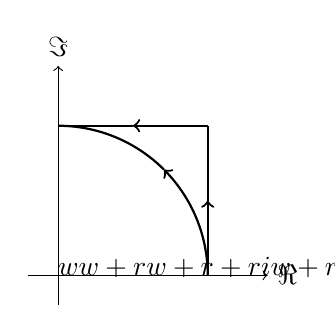
\begin{tikzpicture}[scale=1.9]
        % Axes
        \draw[->] (-0.2,0) -- (1.4,0) node[right] {$\Re$};
        \draw[->] (0,-0.2) -- (0,1.4) node[above] {$\Im$};
    
        % Quarter-circle contour
        \draw[thick, domain=0:45, ->] plot ({cos(\x)}, {sin(\x)});
        \draw[thick, domain=45:90, -] plot ({cos(\x)}, {sin(\x)});

        % Rectangular contour
        \draw[thick, ->] (1,0) -- (1,0.5);
        \draw[thick, -] (1,0.5) -- (1,1);
        \draw[thick, ->] (1,1) -- (0.5,1);
        \draw[thick, -] (0.5,1) -- (0,1);

        % % Dyadic style approximation
        % \foreach \n in {0, 1, 2, 3, 4, 5, 6, 7, 8, 9, 10} { % Depth
        %     \foreach \l in {1, ..., \n} { % Lines
                
        %     }
        % }

        % Points of interest
        \labelledpoint{0}{0}{-0.3}{-0.8}{$w$}
        \labelledpoint{1}{0}{0}{-0.8}{$w + r$}
        \labelledpoint{1}{1}{0.3}{-0.2}{$w + r + ri$}
        \labelledpoint{0}{1}{-0.7}{-0.5}{$w + ri$}
    \end{tikzpicture}
    \caption{The contours in \Cref{Ch5:Thm:CauchyGoursat_Circle_Rectangle}.}
    \label{Ch5:Fig:Square_Circle_Contour}
\end{wrapfigure}

Again, we are saved from the difficulties of applying the \JCT\ because we are working in a very specific situation where we can explicitly describe $S$. However, proving this result, formally and informally, is significantly more complicated than proving \Cref{Ch4:Thm:CauchyGoursat_Unbounded}. One proof would be to arbitrarily approximate $\gamma$ by squares of exponentially decaying side lengths. For any contour defined in this way, we can show, by inductively applying \Cref{Ch5:Thm:CauchyGoursat_Bounded_on_off_Countable}, that the integral along it equals the integral along the rectangular contour in \Cref{Ch5:Fig:Square_Circle_Contour}. Since these contours converge to $\gamma$ pointwise, it should be possible to show, by \href{https://github.com/leanprover-community/mathlib4/blob/c38c7fde32656c7fa1b2471ed1ae0d50a600f089/Mathlib/MeasureTheory/Integral/DominatedConvergence.lean#L49-L63}{dominated convergence}, that the (constant) sequence of integrals along the square contours converges to the integrals along $\gamma$.

Unfortunately, these ideas are incredibly difficult to formalise, not least because it is difficult to define such a sequence of parametrisations in Lean. Other possible approaches include formalising a version for triangles and subsequently approximating the circle using triangles. Regardless of the approach, formalising \Cref{Ch5:Thm:CauchyGoursat_Circle_Rectangle} will be a challenge. If done successfully, however, it will be a significant achievement in itself as well as a valuable contribution to this project.